\chapter{Evaluation}

Despite the fact, how good the prototype in terms of algorithmic and design approaches. There will be some probability that elaborates, users are doing what they are not expected to do.  This leads to other features(s) that needs to be develop in order to improves the user’s satisfaction and increase his willingness to user the system. Therefore it is important that developed system should go through an evaluation proves before it goes live. Focus of evolutions to ensure that product is appropriate and the involvement of user through the design process. This chapter depicts the evaluation of prototype in a real user study and present the result.

\section{Motivation and Goals}

Motivation behind performing evaluation to determine, whether the process of recipe according to user interest in mobile critique-based recommender system can be improved by applying Persuasive Principles. As discussed earlier, purpose of developed Food Recommender System aim to be used in a real world situation. This established some aspects of the user study, including the development of a variant of the proposed application and assessment of the system.\newline

During the study, two variants of the system will need to be tested, one begin the basic interface design, without explanation and works on basic recommender system by providing star rating to the recipes. Whereas, the second system is the main output of thesis, with better infrastructure of recipes, sleeker interface and having explanation about the recipes. Additionally recommender system algorithm supports critiquing on both ingredients and recipes.\newline 

The study is designed in a way that each user has to test both variants of the application, which system is more appealing for the users. Focusing on real effect of recommendation depends on factors like user intent, context, way to present recommendations set and other. Thus experiment needs to provide evidence as the true value of evaluation.\cite{shani2011evaluating}. Additionally a single irritation of user study should not exceed with more then 20 min to maintain user interest. Considering the fact that user have to test two variant of application. However it is possible that user might have get some less qualitative results which is not due the fault from the system but because users were overwhelmed with long sessions.  \newline

The focus of evaluation was to measure the effect of persuasion by providing the recommendation in form of recipes. Also how active learning also system to change itself according to user preferences. However it exclude the non-relevant part like ingredients integration to improve the recipes.

\section{Data set Generation}

Data sets are necessary to create a pragmatic setup to represent a real world objects. Therefore, a data crawler needs to be developed as an open-source project that will crawl the recipes form any recipe data bank. Crawler developed by us is written in java.  Crawling recipe form data bank is a two steps process.  First fetches the recipes from databank on behave of food type and course.  In second step it will sync all those recipes whose details are not present in our database. Additionally recipes images are not been stored in our system instead of saving image we stores their URLs. Extracted data provide international recipes of different cousins. However, it provides functionally to add more different data source that provides recipes. To keep the amount of work reasonable items were associated with the following:

\begin{enumerate}
	\item Unique identifier for recipes
	\item 11 types of courses (e.g,. Appetizers, Bread)
	\item 91 Cuisine (e.g. American, Thai, Beverages)
	\item Images links of different sizes
	\item Preparation
	\item List of ingredients
	\item Popularity of recipe
\end{enumerate}

Currently our data bank has 1303 of recipes, 10037 ingredients. Furthermore, it can grow more depends on crawling method.

\section{Setup}

This section leads our discussion toward the selection of test hardware, different variants of application and testing framework for the sake of performing evaluation.

\subsection{Test Hardware}

Recommended hardware must have at least 320x 480 resolution and above, running iOS version 8.0 or later. In order words required device to run application is iPhone 4S and above.  

\subsection{Variants}

Two variants of system are developed to test. Both variants use the same recommendation algorithm. However they are different to each other by have unique interface design, explanation of recommendation and critiquing methodology. 

\begin{enumerate}
	\item \textbf{Experiment (EXP)} This variant refers to the proposed developed system as discuss in chapter 4. It allows users to change their preferences while interacting to the system by critiquing on ingredients and recipes. System provides explanation to each recommended item. Additionally interface follows the user centric design, which contains more information about the recipe to draw user attention towards recipes.
	
	\item \textbf{Basic (BASE)}  Consider as baseline to compared the needs and effectiveness of actual system. In this system mostly provides textual information about the recipe. User can critique only recipes by given stars. System does not provide any explanation along with recipes. 
\end{enumerate}

\subsection{Testing Framework}

Testing framework that is applied in user study is a subset of the aspect that are relevant for persuasion and critiquing in recommend system. It follows the user-centric design approaches \cite{pu2006trust} and framework that applied for evaluation of recommend recommendation system \cite{shani2011evaluating}. Measure data is divided into following areas:

\subsubsection{Persuasion’s Principle}

Persuasion’s principle that discussed in section \ref{ch4_persuasion_explaination} were related to the how these factors will be implemented in our system.  It is essential aspect for this thesis that the recommendations that are suggested to user should ne persuasive in nature and follows the principle. The forth-coming discussion relates whether user might be able to perceive those or not.

  \begin{enumerate}
  	\item \textit{Perceived Reciprocity} is allows user to return his favor by critiquing as recipe and select other good food according to particular food course and cuisine. The participants were asked they think that system helps them to select them a recipe although this recipe his according to his preferences, but the system consider other user feedback on that recipes before making up recommendations.
  	
  	\item \textit{Perceived Scarcity} measurement indicates by categorizing recommendation with respect to context and consumption time of recipe. Participants were asked whether they find that system helps them to filter out the recipe according to their meal time.      

  	\item \textit{Perceived Authority} refers to the popularity of a particular recipe in a given context of user. To measure the level of perceived authority, Participants were asked to what ascent they felt authority. 
  	
  	\item \textit{Perceived Liking} refers to factors that include liking a recipe. In our system measure matric was based on ingredients and recipe staring. Participants were asked which mechanism like/dislike help more in finding out the recipe. 	  
  	
  	\item \textit{Perceived Commitment} indicated to what degree system is committed to user preference. In order to measure the degree of commitment metric is defined. Participants were asked to mark if they felt that system is committed to preferences or not.	  
  	  	
  	\item \textit{Perceived Social Proof} denotes the what society think about that particular item in our case recipe. User may or may not thought that social factor is present, By asking the user to what level they consider social factor is present in our system by providing them a scale.   
  \end{enumerate}
  
\subsubsection{Transparency}

Ability of a system that allows user to understand its working and explain system choices and behavior. However it is possible that user’s understanding about the system working might be differ form its actual working. For the sake of evaluation user were asked to mark choices that they think about the system when making recommendations. \newline

\textit{Perceived Transparency:} There is a possibility that user might or not perceive that system is transparent. By asking the factors which users thinks system include while making a recommendation. It is possible learn their perceived transparency.


\subsubsection{User Control}
Level of control that provides to users while operation a system refers to User Control. Under this sub section we want to measure the following items:  \newline

\textit{Perceived Overall Control} indicates that does user have overall control over recommendation. The participant were asked about what they feel about while using the application by rating that were they able to tell about the system which recipes are the looking for, telling their preference to system and finally to what assent they feel they have control over system. \newline

\textit{Perceived Scrutability} denotes the ability of the system that allows user to revised their preference and excludes those assumptions that system made on there behaves. Participants were asked to rate till what ascent they feel control over system to correct the wrong assumption made by the system.

\subsubsection{Efficiency}

Providing good recommendation is not only the task of recommender systems. Also it is essential for a system how quickly it come to decisions that help in selection of item especially in the domain of mobiles. Measuring efficiency is divided into two perspectives. First, as in conversational recommender numbers of cycles were counter.  Where each cycle defined as number of times user have to perform update his preference in order to complete a task. Each cycle have an impact on user model. Second refers as time that passed from display of first recommendation set to selection and confirmation of required item. Where time measure in seconds.\newline

\textit{Perceived Efficiency} Duration of item until item found is hard to perceive for user. Therefore for the sake of simplicity user were asked if it requires to much effort to find a recipe they are looking for. Additionally run of cycles are also hard to reminder but since conversation system cycle normally cycle are not be exceed to two cycle. Therefore user were asked to mention in which cycle they received their recipe. 

\subsubsection{Satisfaction}

Satisfaction is the ability to make system fun while user is interacting with the system. Also providing poor recommendation decrease the user interest.\newline

\textit{Perceived Satisfaction} measure to determine user’s feeling while in using system. It allows user to express their preferences about the system in a direct way. Participants were asked to which ascent they were satisfied about they system.

\subsubsection{Context}

Context defines as any information that can be used to characterize the situation of entity. It is important for recommendation to consider the context while making a recommendation in order to make the recommendation more concrete. \newline

\textit{Perceived Context} are determine in following ways: calories information about the recipe, cooking time and course of recipes. Participants were asked to select which contextual information helped them to select to recipe. 

\subsubsection{UserDemographic}

Participants were asked to fill their demographic information for instance age, occupation, how often they cooked. 

\subsection {Testing Procedure}

Evaluation's testing procedure was structured in the following order:
 \begin{enumerate}
 	
 	\item  Initially participants were asked to provide their background information, which include age, occupation. Additionally they need to provide how often they cooked considered demographic information.
 	
 	\item Next step was to present the idea of system and the purpose of user study to the participant. So they have a clear understanding about both presented items.  
 	
 	\item Instead of requesting user to pick up the random recipe according to their interest present a realistic scenario, which helps user in order to mention their interest like as follows:\newline 
 	
 	\textit{Imagine you just came for gym. You need prepare a meal for yourself. You have prepared a meal according to you taste and diet plan and have an hour for cooking.  You are not sure what to cook. You opened FoodForMe app and start looking what needs to prepare. After you find the recipe you need to provide your feedback.}\newline
 	\textit{For first step your task is:}\newline
 	\textit{Find a recipe you would lie to cook if given the opportunity that satisfies the following:}
 	\begin{enumerate}
	 	\item \textit{Cooking time 90min.}
	 	\item \textit{Type of recipe : Appetizer,  bread, breakfast, salads, soups etc.}
 	\end{enumerate}
 	\textit{After introducing task, hand over the app to users so that familiarize themselves with the interface and app workflow. They were also asked that this task would be executed twice with two different variants of the app, leading to potentially better or worse recommendations. Finally they need to judge which variant is better.}
 	
 	\item After demonstration of task, users need to understand how to perform critique and setup their preferences. 
 	
 	\item Participants were encouraged to given their verbal feedback about the system. Although it'ss not mandatory. All the verbal feedbacks were noted. 
 	
 	\item Once the tester performed his task and selects the recipe, which is satisfied as per his preference. The whole process was repeated for other variant of the system. 

	\item Finally each participant was interviewed about which  variant they liked the most and why by filing a questioner. 

 \end{enumerate}
 
\section{Results}

In this section our discussion leads to the result of data points measures via user study.  

\subsection {Participants}

People who performed evaluation was belong to various age groups and have different occupation. Overall 31 people participated, 24 students, 5 employee, 2 self-employed and 1 is housewife. 78.1\% of them have age between 18 to 35 years.  12.5\% are between 12 to 18 years old. Where people whose ages are above 35 year have a small portion which is 9.4\%. Figure \ref{fig:stat_demographic_info} shows their distribution separately. \newline

	  \begin{figure}[h]
	  	\centering
	  	\begin{subfigure}{.45\textwidth}
	  		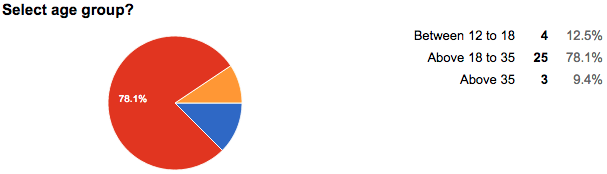
\includegraphics[width=.9\linewidth]{figures/ch5_stat_age.png}
	  		\caption{Participants Age}
	  	\end{subfigure}
	  	\begin{subfigure}{.45\textwidth}
	  		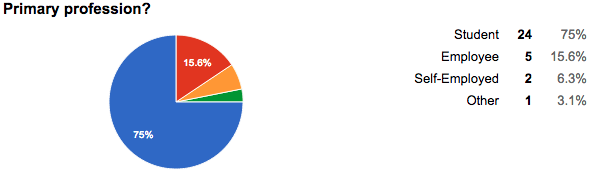
\includegraphics[width=.9\linewidth]{figures/ch5_stat_profession.png}
	  		\caption{Participants Profession}
	  	\end{subfigure}
	  	\begin{subfigure}{.45\textwidth}
	  		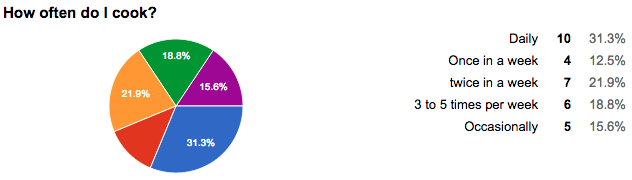
\includegraphics[width=.9\linewidth]{figures/ch5_stat_cook.png}
	  		\caption{How much Participants cook}
	  	\end{subfigure}
	  	\caption{Participants Demographic Info}
	  	\label{fig:stat_demographic_info}
	  \end{figure}
	  
Where as in terms of cooking, about 31.2\% of the participants are likely to cook daily, however 21\% of them cook twice a week and 18.8\% said that they need to cook 3 to 5 timer per week and rest are those how cook occasionally.

\subsection{Perceived Persuasion}

Significant change in user’s intension to cook a recipe has been observed form the result. To determine which strategies preform better in terms of persuasiveness, paired t-test were used upon the difference between initial rating and the one for each strategy. The results in Table \ref{table:persusasion-result} reflects the effectiveness comparison among the strategies. 

\begin{table}[ht]
	\centering % used for centering table
	\begin{tabular}{p{2cm} p{2cm} p{2cm} p{2cm} p{2cm} p{2cm}}
		\hline\hline %inserts double horizontal lines
		& Scarcity & Authority & Social Proof & Liking & Commitment\\ % inserts table
		%heading
		\hline % inserts single horizontal line
		Reciprocity   & <0.001  & <0.001 & <0.001 &  0.083 & <0.001 \\ % inserting body of the table
		Scarcity      &         & <0.001 &  0.169 & <0.001 & <0.001 \\
		Authority     &         &        &  0.089 & <0.001 &  0.325 \\
		Social Proof  &         &        &        & <0.001 &  0.083 \\
		Liking        &         &        &        &        & <0.001 \\
		Commitment    &         &        &        &        &  \\ [1ex] % [1ex] adds vertical space
		\hline %inserts single line
	\end{tabular}
	\caption{Paired t-test was used to examine significance, where 0.05 is set as the threshold for p-value to evaluate the significance and p-value lower than 0.001 indicates strong significance.}
	\label{table:persusasion-result}
\end{table}


Next we discuss the impact of each of the persuasiveness factor individually and focus on what was the consideration of participant about them.\newline

\subsubsection{Reciprocity}

Selecting which system is most like by user does measurement of Reciprocity. System that provides only textual information was BASE and on the other hand EXP has more information contains all the graphical information about recipes. People are more reluctant towards EXP i.e. 93.8\%. Figure \ref{fig:ch5_stat_reciprocity} represents the reciprocity measurement.

\begin{figure}[h]
	\centering
	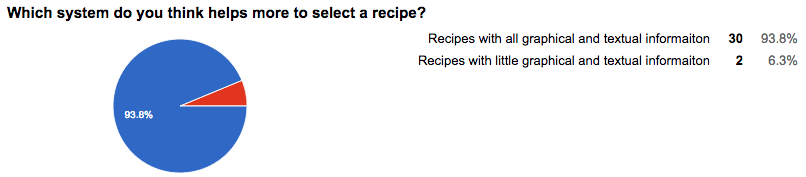
\includegraphics[width=1\linewidth]{figures/ch5_stat_reciprocity}
	\caption{Perceived Reciprocity}
	\label{fig:ch5_stat_reciprocity}
\end{figure}

\newpage
\subsubsection{Scarcity}

Asking the participants what they feel about scarcity by filtering out the recipe with respect to meal by provide the liker scale. Where 1 mean strongly agree and 5 means strongly disagree.  34.3\% of them were quite sure about it and 43.8\% feel good about that. Additionally 15.6\% were moderate about this statement. Where 6.2\% how felt negative about this statement. 
\begin{figure}[h]
	\centering
	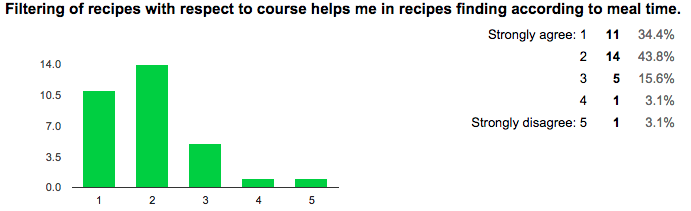
\includegraphics[width=1\linewidth]{figures/ch5_stat_scarcity.png}
	\caption{Perceived Scarcity}
	\label{fig:ch5_stat_scarcity}
\end{figure}

\subsubsection{Authority}

Measuring the authority by asking liker scale question, did they feel that recipe star rating help them in selection of recipe. 93.8\% of participants were positive about that. Conversely people how negate that statement were 6.2\%. Figure\ref{fig:ch5_stat_authority} represents overall statics. 

\begin{figure}[h]
	\centering
	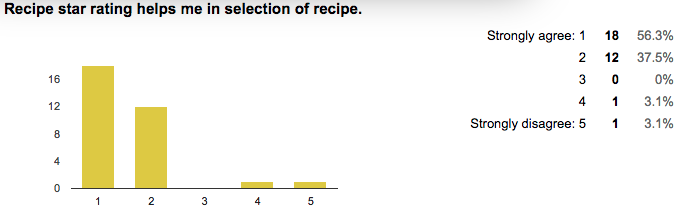
\includegraphics[width=1\linewidth]{figures/ch5_stat_authority}
	\caption{Perceived Authority}
	\label{fig:ch5_stat_authority}
\end{figure}

\subsubsection{Liking}

When ask the participants which recipe critiquing technique helps them in finding their recipe. Majority of them voted for critiquing on both ingredients and recipe which in 78.1\%. On the hand minor portion of the participant i.e. 21.9\% liked the conventional critiquing technique to provide their feedback.

\begin{figure}[h]
	\centering
	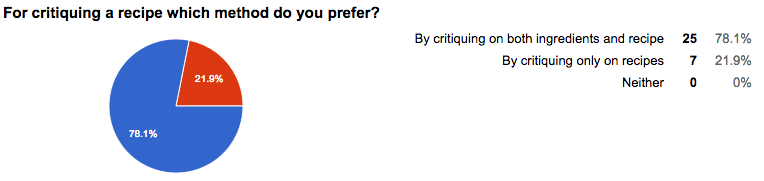
\includegraphics[width=1\linewidth]{figures/ch5_stat_liking.png}
	\caption{Perceived Liking}
	\label{fig:ch5_stat_liking}
\end{figure}

\subsubsection{Commitment}

Participants considered the commitment by providing their answers to liker scale question. In which they have to mention, do they feel explanation of recipe helped them in recipe selection. 90.7\% believed in that statement. Conversely, minor amount of dined to the statement. Where as only 3.1\% were neither agree nether dined to the statement. Figure \ref{fig:ch5_commitment} shows the feedback.

\begin{figure}[h]
	\centering
	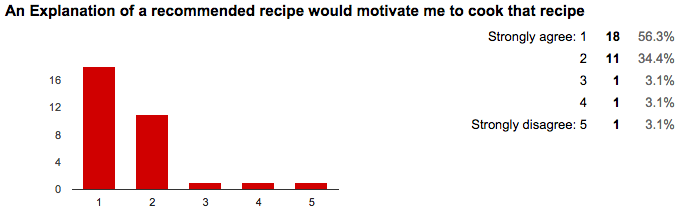
\includegraphics[width=1\linewidth]{figures/ch5_stat_commitment}
	\caption{Perceived Commitment}
	\label{fig:ch5_commitment}
\end{figure}

\subsubsection{Social Proof}

Social proof was measured by asking a likert scale question. In which they had to answered whether participant agreed that he understand that rating a recipe not only helps him to receive better recommendations but also the whole community. 84.4\% of participant were positive and endorsed this fact. In contrast to that a small spike in Figure \ref{fig:ch5_stat_social_proof} represents to those 12.5\% participants how were not favor to that. 

\begin{figure}[h]
\centering
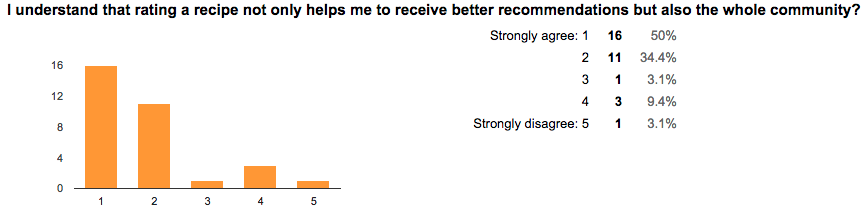
\includegraphics[width=1\linewidth]{figures/ch5_stat_social_proof.png}
\caption{Perceived Social Proof}
\label{fig:ch5_stat_social_proof}
\end{figure}

\subsection{Perceived Transparency}

Once the user performs their task they were asked about how the underlying recommendation system variants work to measure transparency effect. In general, the percipients were able to explain that based on their preferences system builds a there model in each cycle and generate a recommendation for them.  While observing the result there is no clear distinction between the variants. In general, participants felt EXP is more transparent then BASE.  Mean average of EXP is  compared to  the BASE. Further analysis suggested that EXP that provides explanation perceived to more transparent (one-tail t-test, p<0.05 with p=0.018). Figure \ref{fig:ch5_stat_transpancy} shows the rating distribution between two variants. It can be seen clear that in EXP people are more satisfied with respect to BAES. Although there are some participant how feel that system is complex. 


\begin{figure}[h]
	\centering
	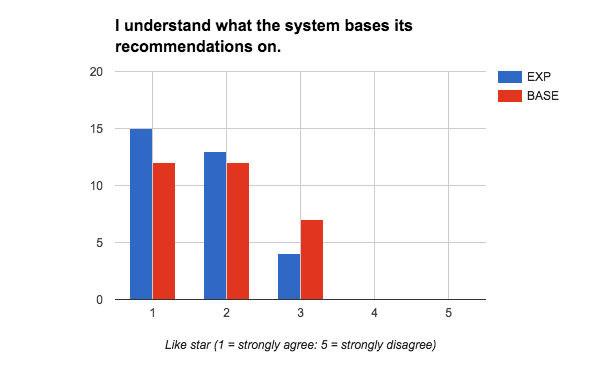
\includegraphics[width=1\linewidth]{figures/ch5_stat_transpancy.png}
	\caption{Perceived Transparency}
	\label{fig:ch5_stat_transpancy}
\end{figure}
\subsection{Perceived User Control}

In our earlier discussion in this chapter, to measure the effect of user control we divided into overall control and suitability perceived by user. 

\subsubsection{Overall Control}

To observe that user were able to perceived overall control or not. They asked about did they felt control while telling the system what they want.  Mean average of EXP is --- where BASE = --. Also further analysis proves that EXP seems to be significantly better than BASE (one-tail t-test, p> 0.05 with p = 0.ddd). Figure \ref{} reflects the actual distribution of rating. Where EXP has \% over positive rating, where there are some percentage of people feel neutral about system where \% doesn’t feel control. 

\subsubsection{Scrutability}

Scrutability measured by asking the user did they feel ease of correcting mistake made by system. EXP performs a lot better than BASE. Mean average of EXP = ,, and BASE --. On more analysis result also support that Scrutability is perceived on EXP than BASE.(One-tail t-test, p<0.05 with p = ). 
Actual distribution of rating in Figure \ref{} reveals the significance of EXP over BASE. 


\subsection{Efficiency}

Efficiency is measured by analyzing the number of critiquing cycle (number of user updates to the preferences by the mean of critiquing). 

\subsubsection{Cycles}
 Participants were asked to mention in which cycle they felt they had received their item.  On average participants completed their task in min 3 cycles before.  EXP mean average  = and BASE  = . However one-tail t-test suggested that EXP is more significant than BASE( p< 0.05 with p = ). Figure \ref{} illustrates the number of cycles that users had performed to complete their task. 

\subsubsection{Perceived Efficiency}

Participants were asked about whether they felt that find the recipe requires too much effort for them. The participants felt satisfaction about the EXP. Average rating got by EXP is … and BASE …. One-tail t-test result also in the favor of EMP where p <0.05 with p= . Figure \ref{} reflects the user choice how they perceived the efficacy in both systems.

\subsection{Perceived Satisfaction}

Satisfaction is measures by inquiring users about their though while interacting with the systems. EXP have better results then EXP by having average of … against .. . by looking at one-tail t-test result we conclude that results are significant (p< 0.05 with p=0.00). Analyzing the rating distribution in Figure \ref{} make it more clear. 

\subsection{Perceived Context}

Participants were asked which contextual information they considered more while selecting a recipe according to preferences. Contextual factors are categories in two major section Calories information, which further divided calories, contains by recipe itself and amount of exercise need to bee done to burn such calories. On the hand context like cooking time and course of the recipe are consider. Considering the result showing in Figure \ref{fig:ch5_stat_context} participants that consider calories information in their diet are 75\% which is majority of population. While more then half population of participant considers recipe course and preparation of recipe. 

\begin{figure}[h]
	\centering
	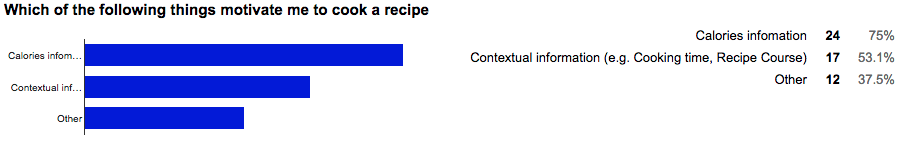
\includegraphics[width= 1\linewidth]{figures/ch5_stat_context}
	\caption{Perceived Context}
	\label{fig:ch5_stat_context}
\end{figure}

\subsection{Informal Feedback}

Our user study was not about feeling questionnaire, Informal feedback given by participant were also encourage and considered as valuable. It is important mention that each feedback was taken separately to each user based on their experience with other apps. Mainly user feedback were around what they feel are missing in our system and existing once. However it fairly possible that other may disagree with these options. Our discussion in this section focuses on most mentioned and participant’s interest feedback. \newline

\subsubsection{Explanation Enhancements}

 	\begin{itemize}
 		\item Some participants mentioned that it would be more helpful for them if the context in a explanation are highlight. It will allow them to take a decision without closely reading the whole paragraph.
 		
 		\item  While some people think that it would be great if explanation of tells recipe us about how does it taste for instances bitter, spicy, mild. 
 		
 		 \item Additionally, fewer people said that it would be nice to have origin of recipe in explanation part. Although it has been shown on top header but considered this section, they accept all the information about the recipe. 
 	\end{itemize}
 	
\subsubsection{More Attributes}

	\begin{itemize}
		\item Majority of participants suggested after seeing calories information in explanation section, they would love to have a feature that would keep track of deity information by allowing them to set a target like how much they want to put on or lose weight.
		 
		 \item Some participant added the above clause by suggesting that there should be a mechanism that will recommend us a weekly diet plan.
		 
		 \item Fewer participants were raised thought that app should consider also what ingredient they have and what recipes they can cook along with that items. 

		\item In addition to above point 1 or 2 participants suggested idea the app will attract them more if they can edit a recipe and contribute their recipes to the system. 

	\end{itemize}

\subsubsection{Endless set of recommenadations}

Quite few users reported, instead of given them specific amount recipes it would be quit helpful if app should provide a pagination functionality so that they can scroll and are able to more and more recipes. By providing us examples of some available products.
	
\subsubsection{Allow sorting}
Fewer participants felt that the app should allow them a functionality to sort the recipes according to type for example, sorting based on popularity and reviews.\newline

Finally, it was observed that as if there are so many ingredients that are liked by users, he can get much or more specific result with critiquing again, that he or she looking for because of limit amount of item set. To solve this problem user should provided endless recommendation set.

\subsection{User Preferences}

Last part of evolution was to ask the participant which variant they liked most why. More then 90\% of participants were in the favor of EXP over BASE. Reasons were BASE has allowed them to critique only the recipes because of this critiquing cycles were increased to 2X to 3X. Furthermore, participants liked to know what the system thinks about their preference and why this recommendation is for them EXP allows them where BASE don’t. Last but no the least only providing the recipes details is not sufficient for user, People want more and more information about the item which they select the more information they have the better they previse. 

	  \begin{figure}[h]
	  	\centering
	  	\begin{subfigure}{.80\textwidth}
	  		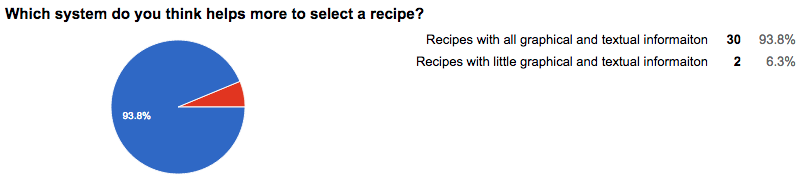
\includegraphics[width=.9\linewidth]{figures/ch5_stat_user_preference_recipe_info}
	  		\caption{Recipe Information}
	  	\end{subfigure}
	  	\begin{subfigure}{.80\textwidth}
	  		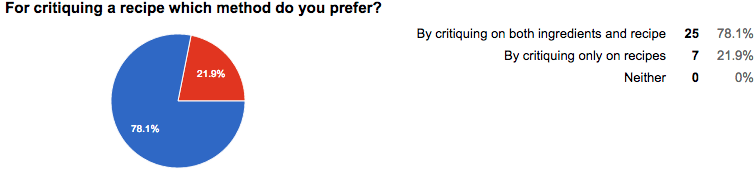
\includegraphics[width=.9\linewidth]{figures/ch5_stat_user_preference_recipe_critique}
	  		\caption{Recipe Critique}
	  	\end{subfigure}
	  	\begin{subfigure}{.80\textwidth}
	  		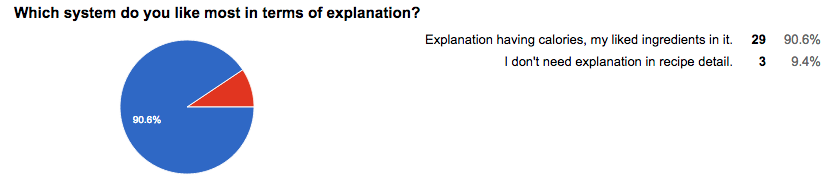
\includegraphics[width=.9\linewidth]{figures/ch5_stat_user_preference_recipe_explanation}
	  		\caption{Explanation}
	  	\end{subfigure}
	  	\caption{User Preferences}
	  	\label{fig:ch5_stat_user_preference}
	  \end{figure}
	  
\section{Discussion}

After elaborating on the measurements, now each point will be further analyzed to explain the observed results and share the lessons learned for future improvements. \newline

Starting our discussion with persuasion, EXP has more positive feedback compared to BASE. As per results 90\% of participants in the favor of EXP. Let’s narrow down the discussion to each Principe of Persuasion.  EXP achieved more then 93\%\ of \textit{Reciprocity} than BASE. Participant thinks that preferred information that requires selecting a recipe should contains other review about the recipes and user-centric approach, which involved all textual and graphical information about the recipes.  Overall \textit{Scarcity} is achieved by the system s 78.8\% by filtering out the recipes with respect to consumption time. \textit{Authority} is perceived by 93.8\%, participants feel star rating helps them in recipe selection. \textit{Liking} 78.1\% people in the favor of EXP which means they want to critique on recipe as well as ingredients. EXP leads BASE in terms \textit{Commitment}, 90.7\% of user thought that explanation of recipe motivate them to cook the recipe. Lastly, 
\textit{Social Proof} achieves 84.4\%. Overall looking into the result, we can draw our conclusion that EXP is far more persuasive then BASE. However in order to system more persuasive system should consider more health factors. \newline

In terms of transparency, both system performs well there is no clear winner. Considering the fact system is simpler when it allows small number of items to critique on. However by looking into the results of conducted serve, mostly participant were able to tell the system’s behavior. Moreover, EXP seemed to be transparent to participants, because it provides an explanation. In this case we can draw a conclusion that EXP is superior than BASE. \newline

User felt more control over EXP because it provides explanation through which user could grab an idea what factors are involved in making this recommendation. In addition to EXP allows user to correct the wrong assumption that has been made by the system, which relates to the goal scrutablility. While in BASE it was pretty hard to correct the wrong assumption since it dealt which overall weight of the recipes. \newline

Efficiency has been observed in two ways number of critique cycle that user need to perform to get the particular recipe and overall efficiency of the system in which we measured how much efforts required for a user to find a recipe. In terms of number of cycles EXP provide more efficient result in shorter number of cycle than BASE. Since the critiquing criteria followed by BASE is easy but lead to large number of cycle. Where as intuitive critiquing design of EXP allow users to critique on recipes as well as ingredients which lead to shorter critiquing cycle and far better result then BASE. However people find system is efficient in both variant in finding recipes but comfortable in EXP more than BASE. This might due explanation and over all improved design. \newline

Level of satisfaction of EXP user is remarkably higher than BASE. Although both variants got the positive feedback but due to slick and user-centric design of EXP, its immediately captures the user attention.\newline


Considering the contextual information about the recipe. It seemed like people are more focus towards that system which include calories information along with cooking time and course selection. BASE has got 53.1\% of positive comment but EXP wins again by gain 23\% more votes then BASE. Overall votes for EXP were 75\%.  

Overall, participant prefers EXP over BASE and found more persuasive in nature. Users were comfortable about the explanation about the system and want some more information in it. They found system transparent, efficient, satisfied and provide significant control to them. However, to make system more appealing some changes need to be implemented which includes, consideration of health, sorting, pagination in recommendation list.  